% Arbeitsblatt 1 – Technologies that change society (Spot on facts, pp. 226–227)
% Übersetzen: xelatex ab-1-technologies.tex (zweimal)
% ============================================================
% ab-vorlage.tex – gemeinsame Vorlage der Arbeitsblätter
% englisch/13/questions-on-the-text/arbeitsblaetter/
% Übersetzen mit:  xelatex <datei>.tex   (zweimal, wegen Seitenzahlen)
% Lösungsfassung:  Einzeiler-Datei <datei>-lsg.tex mit
%                  \def\mitloesung{}\input{<datei>}
% Schriften: Carlito (Fließtext), Poppins (Überschriften), TeX Gyre Pagella (Texte)
% ============================================================
\documentclass[10pt,a4paper]{article}
\usepackage[a4paper,top=12mm,bottom=13mm,left=14mm,right=14mm,headsep=4mm,headheight=12pt,footskip=7mm]{geometry}
\usepackage{fontspec}
\setmainfont{Carlito}
\newfontfamily\headfont{Poppins}[UprightFont=* Medium, BoldFont=* Medium]
\newfontfamily\headlight{Poppins Light}
\newfontfamily\lorafont{TeX Gyre Pagella}
\usepackage{xcolor}
\definecolor{prim}{HTML}{2563EB}
\definecolor{primdark}{HTML}{1E3A8A}
\definecolor{sec}{HTML}{7C3AED}
\definecolor{primtint}{HTML}{EFF6FF}
\definecolor{sectint}{HTML}{F5F3FF}
\definecolor{ink}{HTML}{1E293B}
\definecolor{muted}{HTML}{64748B}
\definecolor{rule}{HTML}{CBD5E1}
\definecolor{good}{HTML}{059669}
\definecolor{goodtint}{HTML}{ECFDF5}
\definecolor{warn}{HTML}{B45309}
\definecolor{warntint}{HTML}{FFFBEB}
\definecolor{bad}{HTML}{B91C1C}
\definecolor{badtint}{HTML}{FEF2F2}
\color{ink}
\usepackage[most]{tcolorbox}
\usepackage{tikz}
\usetikzlibrary{positioning,calc,arrows.meta,shapes.misc}
\usepackage{enumitem}
\setlist{nosep,leftmargin=1.1em,topsep=1pt}
\setlist[itemize]{label=\textcolor{prim}{\small\textbullet}}
\usepackage{tabularx,array,booktabs,colortbl}
\usepackage{multicol}
\usepackage{fancyhdr}
\usepackage{lastpage}
\usepackage{amssymb}
\usepackage{microtype}
\setlength{\parindent}{0pt}
\setlength{\parskip}{0pt}
\linespread{1.02}

% ---------- Kopf- und Fußzeile ----------
\newcommand{\wskopf}{English · Q13 · Science and Technology}
\pagestyle{fancy}
\fancyhf{}
\renewcommand{\headrulewidth}{0pt}
\fancyhead[L]{\footnotesize\headlight\textcolor{muted}{\wskopf}}
\fancyhead[R]{\footnotesize\headlight\textcolor{muted}{Name: \rule{38mm}{0.3pt}\quad Date: \rule{18mm}{0.3pt}}}
\fancyfoot[L]{\scriptsize\textcolor{muted}{edu-mrh.de/englisch/13/questions-on-the-text}}
\fancyfoot[R]{\scriptsize\textcolor{muted}{\thepage\,/\,\pageref*{LastPage}}}

% ---------- Titel ----------
% \wstitel{Kürzel}{Titel}{Untertitel}
\newcommand{\wstitel}[3]{%
  \begin{tcolorbox}[enhanced,colback=prim,colframe=prim,arc=2mm,boxrule=0pt,
     left=4mm,right=4mm,top=2.2mm,bottom=2.2mm,
     interior style={left color=primdark,right color=sec}]
    \color{white}{\headlight\footnotesize #1}\\[0.3mm]
    {\headfont\LARGE #2}\\[0.6mm]
    {\small #3}
  \end{tcolorbox}\vspace{1mm}}

% ---------- Boxen ----------
% \begin{wsbox}{Nummer}{Überschrift} ... \end{wsbox}
\newtcolorbox{wsbox}[3][]{enhanced,breakable,colback=white,colframe=rule,boxrule=0.5pt,arc=1.5mm,
  left=2.5mm,right=2.5mm,top=1.3mm,bottom=1.3mm,
  title={\headfont\normalsize\textcolor{white}{\colorbox{prim}{\,#2\,}}\;\textcolor{ink}{#3}},
  coltitle=ink,colbacktitle=white,attach title to upper={\par\vspace{0.6mm}},before skip=1.4mm,after skip=1.4mm,#1}
\newtcolorbox{tintbox}[1][]{enhanced,colback=primtint,colframe=primtint,boxrule=0pt,arc=1.2mm,
  left=2mm,right=2mm,top=1.2mm,bottom=1.2mm,#1}
\newtcolorbox{secbox}[1][]{enhanced,colback=sectint,colframe=sectint,boxrule=0pt,arc=1.2mm,
  left=2mm,right=2mm,top=1.2mm,bottom=1.2mm,#1}
\newtcolorbox{goodbox}[1][]{enhanced,colback=goodtint,colframe=goodtint,boxrule=0pt,arc=1.2mm,
  left=2mm,right=2mm,top=1.2mm,bottom=1.2mm,#1}
\newtcolorbox{warnbox}[1][]{enhanced,colback=warntint,colframe=warntint,boxrule=0pt,arc=1.2mm,
  left=2mm,right=2mm,top=1.2mm,bottom=1.2mm,#1}
\newtcolorbox{badbox}[1][]{enhanced,colback=badtint,colframe=badtint,boxrule=0pt,arc=1.2mm,
  left=2mm,right=2mm,top=1.2mm,bottom=1.2mm,#1}

\newcommand{\kl}[1]{{\headfont\small\textcolor{prim}{#1}}}      % kleine Zwischenüberschrift
\newcommand{\klsec}[1]{{\headfont\small\textcolor{sec}{#1}}}
\newcommand{\plus}{\textcolor{good}{\textbf{+}}\ }
\newcommand{\minus}{\textcolor{bad}{\textbf{–}}\ }
\newcommand{\pfeil}{\textcolor{prim}{$\rightarrow$}\ }
\newcommand{\linie}[1][\linewidth]{\rule{#1}{0.3pt}}
% ---------- Lösungsschalter ----------
% \lsg[Breite]{Text}        Lücke mit Unterstrich; Lösung erscheint nur mit \mitloesung
% \lsglinien{n}{Text}       n Schreiblinien; Lösung wird auf die Linien geschrieben
% Beide reservieren in beiden Fassungen exakt denselben Platz.
\newif\ifloesung
\ifdefined\mitloesung \loesungtrue \else \loesungfalse \fi
\newcommand{\lsgstil}{\color{sec}\itshape}
\newcommand{\lsg}[2][30mm]{%
  \makebox[#1][l]{\rlap{\raisebox{-0.8mm}{\textcolor{rule}{\rule{#1}{0.4pt}}}}%
  \ifloesung{\lsgstil\small #2}\fi}}
\newlength{\lsgzeile}\setlength{\lsgzeile}{7mm}
\newcommand{\lsglinien}[2]{%
  \par\noindent
  \begin{tikzpicture}[x=1mm,y=1mm]
    \pgfmathsetmacro{\hoehe}{#1*7}
    \path[use as bounding box] (0,0.5) rectangle (\linewidth,-\hoehe);
    \foreach \i in {1,...,#1} {\draw[rule,line width=0.4pt] (0,-\i*7) -- (\linewidth,-\i*7);}
    \ifloesung
      \node[anchor=north west,inner sep=0pt,text width=\linewidth,align=left,
            font=\lsgstil\small] at (0,-3.3) {\setlength{\baselineskip}{\lsgzeile}#2\par};
    \fi
  \end{tikzpicture}\par}
\newcommand{\schreiblinien}[1]{\lsglinien{#1}{}}


\begin{document}
\fontsize{9.4}{10.9}\selectfont

\wstitel{Worksheet 1 · Spot on facts, pp.\,226–227}{Technologies that change society}%
{The facts at a glance — your foundation for the Kolloquium and for any factual text on science and technology.}

% ------------------------------------------------------------------ 1
\begin{wsbox}{1}{Developments in the 21st century}
\begin{tabularx}{\linewidth}{@{}>{\raggedright\arraybackslash}X@{\hspace{3mm}}>{\raggedright\arraybackslash}X@{\hspace{3mm}}>{\raggedright\arraybackslash}X@{}}
\kl{Genetic engineering} & \kl{Eco-technology} & \kl{AI \& digital content}\\
\textbf{CRISPR} = tool that \emph{precisely edits} the genetic code of organisms. &
Ocean clean-ups try to remove the ever-growing amount of plastic waste. &
Large language models turn \emph{prompts} into texts, audiovisual content and complex programs.\\[0.3mm]
\plus drought-resistant crops; better treatments for incurable diseases (e.g.\ stem cells from human embryos) &
\plus solar, hydrogen and wind power are more affordable and efficient; the share of electric vehicles is rising &
\plus masses of information and data can be re-used in myriad contexts\\[0.3mm]
\minus morality of the research; risks of human \emph{interference} with DNA &
\minus fossil-fuel cars still outnumber e-cars in most countries; \emph{raw materials} (lithium, rare-earth metals for batteries) create new environmental problems &
\minus often impossible to know where content comes from and how trustworthy it is
\end{tabularx}
\end{wsbox}

% ------------------------------------------------------------------ 2
\begin{wsbox}{2}{Artificial intelligence (AI)}
\begin{tintbox}
\textbf{Definition:} AI is \emph{the simulation of human intelligence in machines} — learning, problem-solving, \emph{reasoning} and perceiving. The field \emph{encompasses} anything from online search engines to military weapons and is progressing rapidly.
\end{tintbox}\par\vspace{1mm}
\begin{minipage}[t]{0.47\linewidth}
\begin{tabularx}{\linewidth}[t]{@{}>{\raggedright\arraybackslash}X@{\hspace{2mm}}>{\raggedright\arraybackslash}X@{}}
\kl{Weak / narrow AI} & \kl{Strong / general AI}\\
single-task oriented, e.g.\ personal assistants, video games &
more complex, human-like, e.g.\ (book) self-driving cars, robotic systems
\end{tabularx}\par\vspace{0.8mm}
{\footnotesize\textcolor{warn}{\textbf{Careful:}} most experts today use \emph{general AI} (AGI) for a still hypothetical AI with human-level intelligence in \emph{all} tasks and count self-driving cars as narrow AI.}\par\vspace{0.8mm}
\pfeil \textbf{Key consequence:} checking data and recognising manipulation matter more than ever — for individuals, companies and governments.
\end{minipage}\hfill
\begin{minipage}[t]{0.5\linewidth}
\kl{Impact on society}\par\vspace{0.3mm}
\begin{itemize}
\item[\plus] benefits everyday life, education and health care
\item[\plus] testing and scrutiny (e.g.\ combining research from diverse sources) can reduce \emph{bias}, improve faulty systems and make slow processes far more efficient
\item[\minus] affects human employment
\item[\minus] ethical questions: telling human from AI texts, video \emph{deepfakes}
\item[\minus] manipulation, misinformation, copyright infringements
\end{itemize}
\end{minipage}
\end{wsbox}

% ------------------------------------------------------------------ 3
\begin{wsbox}{3}{Augmented reality (AR) and virtual reality (VR) — both types of extended reality (XR)}
\renewcommand{\arraystretch}{1.12}
\begin{tabularx}{\linewidth}{@{}>{\raggedright\arraybackslash}p{17mm}>{\raggedright\arraybackslash}X>{\raggedright\arraybackslash}X@{}}
 & \kl{Augmented reality (AR)} & \kl{Virtual reality (VR)}\\\arrayrulecolor{rule}\midrule
What it does & \emph{superimposes} interactive digital elements (visual \emph{overlays}, haptic feedback, sensory projections) on the real world \pfeil \emph{alters} our perception of it & \emph{replaces} our perception of the real world with a computer-generated 360° environment, fully \emph{immersive} or non-immersive\\
Devices & devices with cameras (e.g.\ smartphone, tablet) & headset and motion controllers; simulators\\
Used in & entertainment, medicine, other commercial industries & gaming, marketing, tourism, education, medicine, \emph{warfare}\\
Concerns & data extracted by XR companies & may affect a person's perception of reality; data extraction\\
\end{tabularx}\par\vspace{0.3mm}
{\footnotesize Our texts: Virtual Helsinki = VR tourism (Baxter, p.\,230) · mind uploading = a “virtual afterlife” (Graziano, p.\,234)}
\end{wsbox}

% ------------------------------------------------------------------ 4
\begin{wsbox}{4}{Utopia or dystopia — where will technology take us?}
\begin{minipage}[t]{0.49\linewidth}
\begin{goodbox}
\kl{\textcolor{good}{Utopia}} \enspace Greek \emph{ou} (not) + \emph{topos} (place) = “no place”; sounds like \emph{eu} (good) = “good place”.\par
Coined by \textbf{Thomas More} in 1516: the perfect island of his book could never really exist.\par
\pfeil an \textbf{imaginary, ideal society}; by highlighting aspects of a better world it \emph{criticises contemporary society} and suggests changes.
\end{goodbox}
\end{minipage}\hfill
\begin{minipage}[t]{0.49\linewidth}
\begin{badbox}
\kl{\textcolor{bad}{Dystopia}} \enspace Greek \emph{dys-} (bad) + \emph{topos}.\par
Also political: a \textbf{critique of contemporary socio-political realities} that shows how bad things \emph{could} become — worst-case scenarios if issues stay unaddressed.\par
\pfeil often set in the \textbf{not-too-distant future}, in societies readers recognise; themes: politics, economics, identity, privacy, freedom, health, science and technology.
\end{badbox}
\end{minipage}
\par\vspace{1.2mm}
% Zeitleiste (ordinal, nicht maßstäblich)
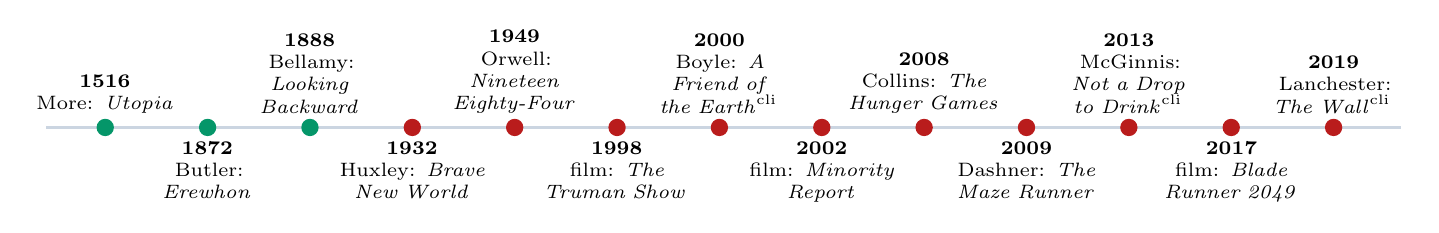
\begin{tikzpicture}[x=1mm,y=1mm,font=\scriptsize]
  \draw[rule,line width=1.2pt] (2,0) -- (174,0);
  \foreach \x/\jahr/\titel/\farbe/\oben in {
    9.5/1516/More: \emph{Utopia}/good/1,
    22.5/1872/Butler: \emph{Erewhon}/good/0,
    35.5/1888/Bellamy: \emph{Looking Backward}/good/1,
    48.5/1932/Huxley: \emph{Brave New World}/bad/0,
    61.5/1949/Orwell: \emph{Nineteen Eighty-Four}/bad/1,
    74.5/1998/film: \emph{The Truman Show}/bad/0,
    87.5/2000/Boyle: \emph{A Friend of the Earth}\textsuperscript{cli}/bad/1,
    100.5/2002/film: \emph{Minority Report}/bad/0,
    113.5/2008/Collins: \emph{The Hunger Games}/bad/1,
    126.5/2009/Dashner: \emph{The Maze Runner}/bad/0,
    139.5/2013/McGinnis: \emph{Not a Drop to Drink}\textsuperscript{cli}/bad/1,
    152.5/2017/film: \emph{Blade Runner 2049}/bad/0,
    165.5/2019/Lanchester: \emph{The Wall}\textsuperscript{cli}/bad/1} {
    \fill[\farbe] (\x,0) circle (1.1);
    \ifnum\oben=1
      \node[anchor=south,text width=19mm,align=center,inner sep=1pt] at (\x,1.4) {\textbf{\jahr}\\\titel};
    \else
      \node[anchor=north,text width=19mm,align=center,inner sep=1pt] at (\x,-1.4) {\textbf{\jahr}\\\titel};
    \fi
  }
\end{tikzpicture}\par\vspace{0.3mm}
{\footnotesize \textcolor{good}{●} utopia \quad \textcolor{bad}{●} dystopia \quad \textsuperscript{cli} = cli-fi (climate fiction), a new subgenre \quad · \quad young-adult dystopias boom: you analysed \emph{The Hunger Games} in Q12!}
\end{wsbox}

% ================================================================== Seite 2
\newpage
\wstitel{Worksheet 1 · Task}{Kolloquium Carousel}%
{In Part 2 of the Kolloquium you answer questions on topics from other semesters — no notes, no slides. Train it now.}

\begin{minipage}[t]{0.52\linewidth}
\kl{How it works}\par\vspace{0.5mm}
\begin{enumerate}[label=\textcolor{prim}{\textbf{\arabic*}},leftmargin=1.2em]
\item Form a double circle. \textbf{Inner circle = candidates}, \textbf{outer circle = examiners} (examiners hold this sheet).
\item The examiner reads a card. The candidate thinks for 15 seconds, then answers for about \textbf{2 minutes}.
\item The examiner asks the \emph{follow-up question} (about 1 minute).
\item The examiner scores with the rubric and gives \textbf{two stars and a wish} (1 minute).
\item Outer circle moves one seat on. After two rounds, swap roles.
\end{enumerate}
\end{minipage}\hfill
\begin{minipage}[t]{0.45\linewidth}
\kl{Answer like a candidate: D – E – E – E}\par\vspace{0.8mm}
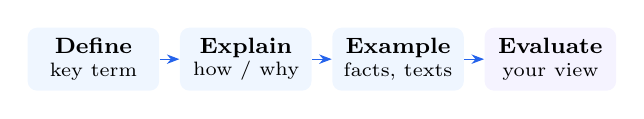
\begin{tikzpicture}[x=1mm,y=1mm,font=\footnotesize,
  stufe/.style={rounded corners=1.2mm,fill=primtint,minimum height=8mm,text width=16mm,align=center,inner sep=1pt}]
  \node[stufe] (d) at (0,0) {\textbf{Define}\\[-0.5mm]{\scriptsize key term}};
  \node[stufe,right=2.5mm of d] (e1) {\textbf{Explain}\\[-0.5mm]{\scriptsize how / why}};
  \node[stufe,right=2.5mm of e1] (e2) {\textbf{Example}\\[-0.5mm]{\scriptsize facts, texts}};
  \node[stufe,right=2.5mm of e2,fill=sectint] (e3) {\textbf{Evaluate}\\[-0.5mm]{\scriptsize your view}};
  \foreach \a/\b in {d/e1,e1/e2,e2/e3} \draw[-{Stealth[length=1.6mm]},prim] (\a) -- (\b);
\end{tikzpicture}\par\vspace{1mm}
{\footnotesize Use the topic words: \emph{to encompass, immersive, to alter, to differ from, interference, sustainable, contemporary, socio-political, issue, prediction}. Link to what you know: our texts, \emph{The Hunger Games}, the news.}
\end{minipage}

\vspace{2mm}
\kl{Question cards}\enspace{\footnotesize\textcolor{muted}{(examiner: pick a card the candidate has not had yet — follow-up in italics)}}\par\vspace{1mm}
\newcommand{\karte}[4]{%
  \begin{tcolorbox}[enhanced,width=\linewidth,colback=white,colframe=rule,boxrule=0.5pt,arc=1.2mm,
     borderline={0.5pt}{0pt}{rule,dashed},left=2mm,right=2mm,top=1.2mm,bottom=1.2mm,height=21mm,valign=center]
    {\headfont\small\textcolor{prim}{#1}\enspace\textcolor{muted}{#2}}\par\vspace{0.4mm}
    {\small #3}\par\vspace{0.4mm}
    {\footnotesize\itshape\textcolor{sec}{Follow-up:} #4}
  \end{tcolorbox}}
\begin{minipage}[t]{0.495\linewidth}
\karte{1}{AR vs VR}{Explain the difference between augmented and virtual reality and give an example of each.}{Which of the two will change everyday life more — and why?}
\karte{3}{Trust}{Why is it becoming harder to know where online content comes from?}{How can individuals protect themselves against manipulation?}
\karte{5}{Eco-tech}{Is eco-technology the answer to our environmental problems?}{What is the “small print” of electric cars?}
\karte{7}{Dystopia}{Choose a dystopian novel or film you know. Which contemporary issue does it criticise?}{Which technology today could lead to a similar society?}
\end{minipage}\hfill
\begin{minipage}[t]{0.495\linewidth}
\karte{2}{AI}{What is artificial intelligence? Distinguish between weak and strong AI.}{Name one area where AI helps and one where it worries you.}
\karte{4}{Genes}{Outline what CRISPR makes possible and why it is controversial.}{Where would you draw the line — think of “designer babies”.}
\karte{6}{Terms}{Explain where the terms \emph{utopia} and \emph{dystopia} come from and what they mean.}{Why might dystopias be more popular than utopias today?}
\karte{8}{Big picture}{Which technology on the page is the most life-changing?}{How will it affect the lives of your generation's children?}
\end{minipage}

\vspace{2mm}
\kl{Examiner's sheet}\enspace{\footnotesize\textcolor{muted}{0 = not yet · 1 = partly · 2 = mostly · 3 = fully}}\par\vspace{1mm}
\renewcommand{\arraystretch}{1.35}
\begin{tabularx}{\linewidth}{@{}>{\raggedright\arraybackslash}X *{2}{>{\centering\arraybackslash}p{30mm}}@{}}
\arrayrulecolor{rule}\toprule
 & \textbf{Round 1} & \textbf{Round 2}\\
Candidate & \rule{26mm}{0.3pt} & \rule{26mm}{0.3pt}\\\midrule
\textbf{Content} — facts and terms are accurate and precise & \quad /3 & \quad /3\\
\textbf{Structure} — clear line of thought (D–E–E–E), gets to the point & \quad /3 & \quad /3\\
\textbf{Language} — topic vocabulary, range, accuracy, fluency & \quad /3 & \quad /3\\
\textbf{Interaction} — reacts to the follow-up spontaneously and to the point & \quad /3 & \quad /3\\\midrule
\textbf{Total} & \quad /12 & \quad /12\\\bottomrule
\end{tabularx}\par\vspace{1.5mm}
\begin{minipage}[t]{0.495\linewidth}
$\bigstar$\,$\bigstar$ \rule{0.85\linewidth}{0.3pt}\par\vspace{4mm}
\textit{wish} \rule{0.85\linewidth}{0.3pt}
\end{minipage}\hfill
\begin{minipage}[t]{0.495\linewidth}
$\bigstar$\,$\bigstar$ \rule{0.85\linewidth}{0.3pt}\par\vspace{4mm}
\textit{wish} \rule{0.85\linewidth}{0.3pt}
\end{minipage}

\vspace{3mm}
\begin{secbox}
\klsec{After the carousel — your Kolloquium note}\enspace{\footnotesize Which card was hardest for you? Note the facts, terms and one example you would need to answer it well next time.}
\schreiblinien{3}
\end{secbox}

\end{document}
